\documentclass{scrreprt}
\usepackage{listings}
\usepackage{graphicx}
\usepackage[utf8]{inputenc}
\usepackage[english]{babel}
\usepackage{tikz}
\usetikzlibrary{arrows.meta}
\usepackage{array}
\usepackage{longtable}
\usepackage[bookmarks=true]{hyperref}
\hypersetup{
    bookmarks=false,
    pdftitle={Software Requirement Specification - Savoury},
    pdfauthor={Savoury Team},
    pdfsubject={Software Requirements Specification},
    pdfkeywords={SRS, Savoury, Mess Management, React Native, Express, Prisma},
    colorlinks=true,
    linkcolor=blue,
    citecolor=black,
    filecolor=black,
    urlcolor=purple,
    linktoc=page
}%
\def\myversion{1.0 }
\date{}

% ---- TikZ node styles ----
\tikzset{
  box/.style   = {rectangle, rounded corners, draw=black, fill=blue!8,
                  minimum width=3cm, minimum height=1cm, align=center, font=\small},
  actor/.style = {rectangle, rounded corners, draw=black, fill=orange!18,
                  minimum width=3cm, minimum height=1cm, align=center, font=\small},
  store/.style = {rectangle, draw=black, fill=green!12,
                  minimum width=3cm, minimum height=1cm, align=center, font=\small},
  flow/.style  = {-{Latex[length=2.5mm]}, thick},
}

\begin{document}

\begin{flushright}
    \rule{16cm}{5pt}\vskip1cm
    \begin{bfseries}
        \Huge{SOFTWARE REQUIREMENTS\\ SPECIFICATION}\\
        \vspace{1.5cm}
        for\\
        \vspace{1.5cm}
        SAVOURY\\
        \large{Hostel Mess Management System}\\
        \vspace{1.5cm}
        \LARGE{Version \myversion}\\
        \vspace{1.5cm}
        Prepared by : 1. Siddharth Singla (1024170252)\\
        2. Vineet Tripathi (1024170253)\\
        3. Shivansh Sahu (1024170249)\\
        \vspace{1.5cm}
        Course : UCS503 Software Engineering\\
        Thapar Institute of Engineering \& Technology, Patiala\\
        \vspace{1.5cm}
        \today\\
    \end{bfseries}
\end{flushright}

\tableofcontents

% ============================================================
\chapter{Introduction}

\section{Purpose}
Managing a hostel mess manually is error-prone and wasteful. Headcounts
for each meal are hard to estimate, so food is routinely over- or
under-prepared; students who are away still pay for meals they do not
eat; and attendance, billing, and refunds are tracked on paper or
spreadsheets. \textbf{Savoury} is the solution. Savoury is a hostel mess
(dining-hall) management platform that digitises per-meal booking,
counter attendance, and student mess-wallet billing. Its purpose is to
let students opt out of meals they will miss (before a configurable
cutoff), give the kitchen an accurate headcount per meal, record who was
actually served at the counter, and automatically debit each student's
prepaid wallet for the meals they take.

\section{Intended Audience and Reading Suggestions}
This SRS is for developers, project managers, wardens, mess committees,
counter staff, students, evaluators, and testers. It describes the
internal and external, functional and non-functional behaviour of
Savoury. Developers and testers should focus on Chapters~3--4 (System
Features and Non-functional Requirements); wardens, committees, and
evaluators will find Chapters~1--2 (scope, stakeholders, and overall
description) most relevant.

\section{Project Scope}
Savoury creates a shared space for Super Admins, Wardens, Co-Wardens,
Caretakers, Mess Committees, Counter (Mess) Staff, and Students to run a
hostel mess.

A \textbf{Super Admin} bootstraps the system, creates hostels, and
appoints hostel administrators. Each hostel has exactly one \textbf{Warden}
and one \textbf{Co-Warden} (identical powers) and any number of
\textbf{Caretakers}; together they manage menus, notices, headcount,
check-in, and student wallets for their hostel. Wardens and Co-Wardens
additionally create \textbf{Mess Staff} accounts (counter staff who serve
meals); Caretakers cannot.

A \textbf{Student} registers with a college email, is attached to a
hostel, and uses the mobile app. By default every student is assumed to
be eating every meal (\emph{implicit opt-in}); they opt out of specific
days/meals before each meal's cutoff. Students view the menu and notices,
and manage a prepaid \textbf{mess wallet} (top-ups, meal deductions, and
end-of-semester cashout).

At meal time, \textbf{Counter Staff} mark students as served (via roster
or QR). Each serve writes an attendance record and debits the student's
wallet by the meal's per-meal rate in a single transaction; duplicate
serves are rejected.

Figure~\ref{fig:workflow} shows the overall work-flow. The entities are
mutually dependent: students take meals that are planned by the mess
committee, locked by configurable cutoffs, served and billed by counter
staff, and overseen per hostel by wardens, with the whole system
administered by the super admin.

\begin{figure}[h!]
    \centering
    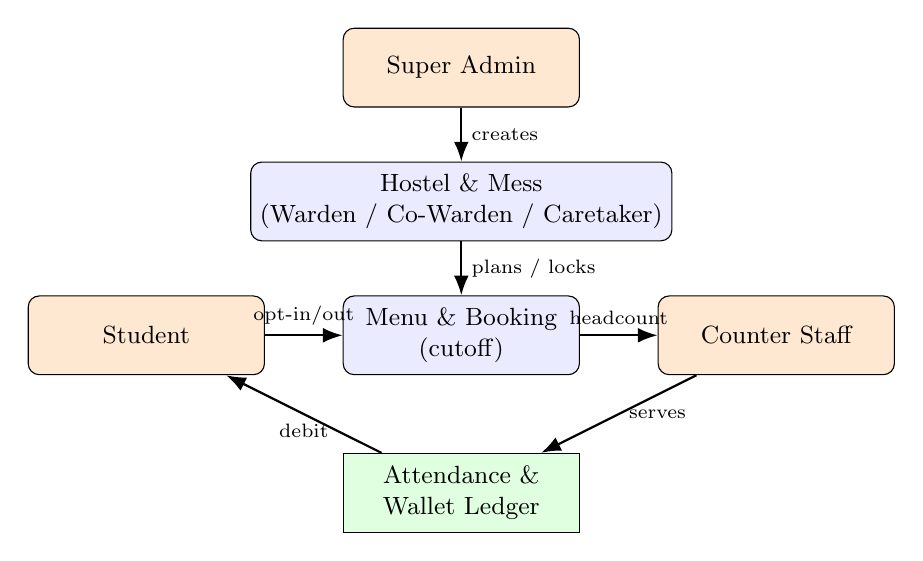
\begin{tikzpicture}
      \node[actor] (sa)      at (0, 6)    {Super Admin};
      \node[box]   (hostel)  at (0, 4.3)  {Hostel \& Mess\\(Warden / Co-Warden / Caretaker)};
      \node[box]   (menu)    at (0, 2.6)  {Menu \& Booking\\(cutoff)};
      \node[actor] (student) at (-4, 2.6) {Student};
      \node[actor] (staff)   at (4, 2.6)  {Counter Staff};
      \node[store] (wallet)  at (0, 0.6)  {Attendance \&\\Wallet Ledger};

      \draw[flow] (sa)     -- node[right,font=\scriptsize]{creates} (hostel);
      \draw[flow] (hostel) -- node[right,font=\scriptsize]{plans / locks} (menu);
      \draw[flow] (student)-- node[above,font=\scriptsize]{opt-in/out} (menu);
      \draw[flow] (menu)   -- node[above,font=\scriptsize]{headcount} (staff);
      \draw[flow] (staff)  -- node[right,font=\scriptsize]{serves} (wallet);
      \draw[flow] (wallet) -- node[below,font=\scriptsize]{debit} (student);
    \end{tikzpicture}
    \caption{Entire work-flow}
    \label{fig:workflow}
\end{figure}

\section{Objectives}
\begin{enumerate}
  \item Provide accurate per-meal headcounts to reduce food wastage.
  \item Let students opt out of meals they will miss, before a cutoff.
  \item Record counter attendance as the single source of truth for billing.
  \item Automate wallet debits per meal and support top-ups and cashouts.
  \item Enforce hostel-scoped, role-based access across all operations.
\end{enumerate}

% ============================================================
\chapter{Overall Description}

\section{Product Perspective}
Savoury replaces the manual, paper-based mess-attendance and billing
process. It is a new, self-contained client--server system comprising a
shared REST backend, a student mobile app, and a staff/admin web console.
The main goal is to minimise manual effort and food wastage while
maximising billing accuracy and transparency for the mess operation.

\section{User Classes and Characteristics}
Savoury has the following classes of users, shown in
Figure~\ref{fig:users}:
\begin{itemize}
  \item Administrators
    \begin{itemize}
        \item Super Admin
        \item Warden / Co-Warden
        \item Caretaker
    \end{itemize}
  \item Mess Committee
  \item Counter (Mess) Staff
  \item Students
\end{itemize}
The Super Admin manages hostels and appoints hostel administrators.
Warden, Co-Warden, and Caretaker share an identical feature set for their
hostel (the only difference: only Warden/Co-Warden may add Mess Staff).
Mess Committee members are students with menu/notice/headcount
privileges. Counter Staff only serve meals and never log in to the mobile
app. Students fulfil registration (college email, hostel) and use the
mobile app.

\begin{figure}[h!]
    \centering
    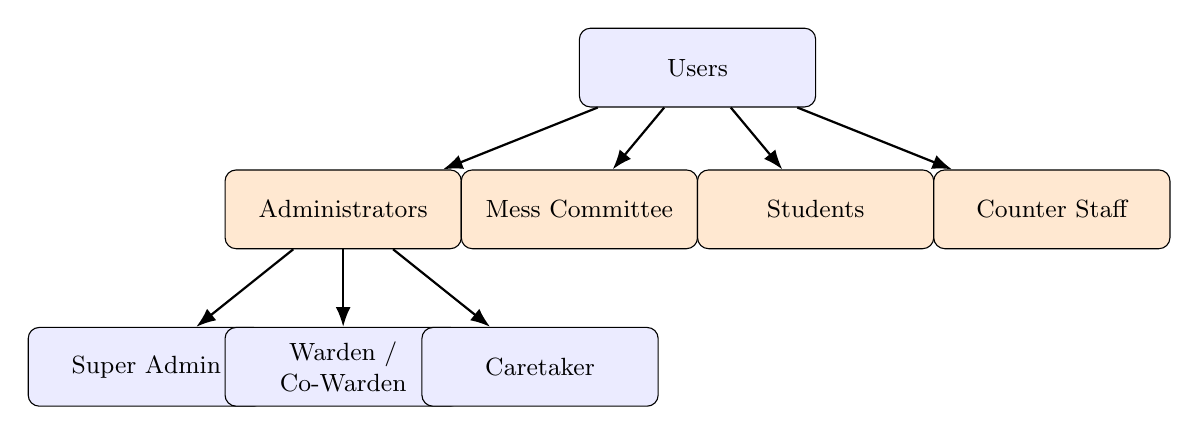
\begin{tikzpicture}
      \node[box]   (users)     at (0, 5)      {Users};
      \node[actor] (admins)    at (-4.5, 3.2) {Administrators};
      \node[actor] (committee) at (-1.5, 3.2) {Mess Committee};
      \node[actor] (students)  at (1.5, 3.2)  {Students};
      \node[actor] (staff)     at (4.5, 3.2)  {Counter Staff};

      \node[box]   (super)  at (-7, 1.2) {Super Admin};
      \node[box]   (warden) at (-4.5, 1.2) {Warden /\\Co-Warden};
      \node[box]   (care)   at (-2, 1.2) {Caretaker};

      \draw[flow] (users) -- (admins);
      \draw[flow] (users) -- (committee);
      \draw[flow] (users) -- (students);
      \draw[flow] (users) -- (staff);
      \draw[flow] (admins) -- (super);
      \draw[flow] (admins) -- (warden);
      \draw[flow] (admins) -- (care);
    \end{tikzpicture}
    \caption{Types of users}
    \label{fig:users}
\end{figure}

\section{Product Functions}
Savoury stores menus, bookings, attendance, and wallet ledgers for all
students of a hostel's mess. Figure~\ref{fig:dfd} is the data-flow
overview.

\begin{figure}[h!]
    \centering
    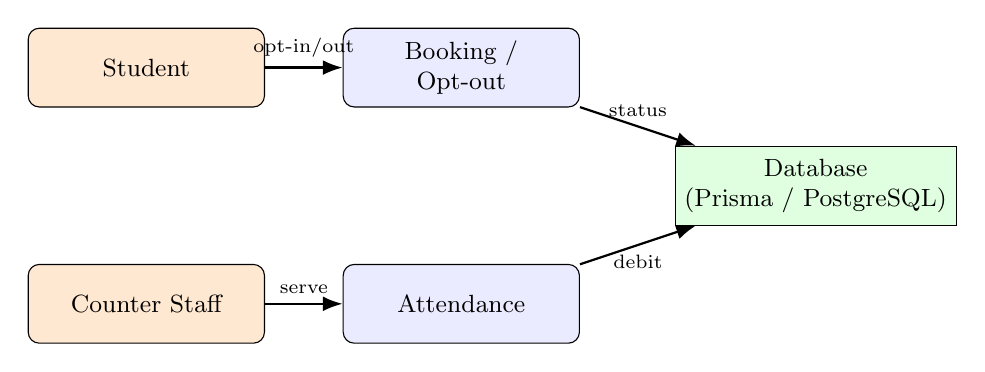
\begin{tikzpicture}
      \node[actor] (student) at (0, 3)   {Student};
      \node[box]   (booking) at (4, 3)   {Booking /\\Opt-out};
      \node[store] (db)      at (8.5, 1.5) {Database\\(Prisma / PostgreSQL)};
      \node[actor] (staff)   at (0, 0)   {Counter Staff};
      \node[box]   (att)     at (4, 0)   {Attendance};

      \draw[flow] (student) -- node[above,font=\scriptsize]{opt-in/out} (booking);
      \draw[flow] (booking) -- node[above,font=\scriptsize]{status} (db);
      \draw[flow] (staff)   -- node[above,font=\scriptsize]{serve} (att);
      \draw[flow] (att)     -- node[below,font=\scriptsize]{debit} (db);
    \end{tikzpicture}
    \caption{Data Flow Diagram}
    \label{fig:dfd}
\end{figure}

Before using the system, users must be authenticated. All users share
these fields: id, name, email, phone, roomNo, avatar, passwordHash, role,
hostelId, createdAt, and updatedAt.

\textbf{Students} additionally carry a unique rollNo and are linked to a
hostel; their eating behaviour is derived from Bookings and Meal Opt-outs
rather than stored explicitly (implicit opt-in).

Each \textbf{Hostel} has one \textbf{Mess} and one or more
\textbf{HostelFeePlan} rows (semesterLabel, totalFee, semesterEndDate).

\textbf{MealType} rows (one per slot: Breakfast, Lunch, Dinner) carry a
displayName, a serving window (servingStart, servingEnd), a
defaultCutoffTime, and a perMealRate (seeded at 75.00).

\textbf{Menu} rows store free-form JSON items per mess, meal, and date.

\textbf{Booking} is the core scheduling entity, unique per
(studentId, mealTypeId, date), with status OPTED\_IN / OPTED\_OUT /
LOCKED and a lockedAt timestamp set by the cutoff cron.

\textbf{Attendance} (unique per bookingId) is the source of truth for
billing, with result SERVED / DUPLICATE / OVERRIDE.

\textbf{WalletAccount} (unique per studentId, semesterLabel) holds the
balance and owns \textbf{WalletTransaction} rows (TOPUP, MEAL\_DEDUCTION,
CASHOUT, ADJUSTMENT); \textbf{CashoutRequest} tracks end-of-semester
refunds.

\section{Operating Environment}
The backend is a Node.js (Express + TypeScript) service with a
PostgreSQL database, deployable on any OS and hosted on Render with a
Supabase database. The web console runs in any modern browser
(Chrome, Firefox, Edge, Safari). The mobile app runs on Android and iOS
via Expo / React Native.

\section{Design}
Student activities follow three steps:
\begin{itemize}
    \item Registration (college email, hostel assignment)
    \item Opt-out planning (before each meal's cutoff)
    \item Profile \& wallet (balance, transactions, cashout request)
\end{itemize}
A student registers, is attached to a hostel, and is thereafter assumed
to eat every meal unless they opt out before cutoff. Their profile shows
personal information, wallet balance and transactions, the menu, and
notices targeted to their hostel/role.

\begin{figure}[h!]
    \centering
    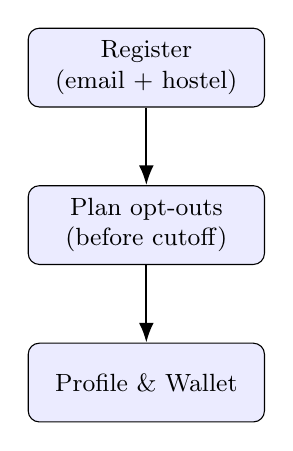
\begin{tikzpicture}
      \node[box] (reg)  at (0, 4) {Register\\(email + hostel)};
      \node[box] (opt)  at (0, 2) {Plan opt-outs\\(before cutoff)};
      \node[box] (prof) at (0, 0) {Profile \& Wallet};
      \draw[flow] (reg) -- (opt);
      \draw[flow] (opt) -- (prof);
    \end{tikzpicture}
    \caption{Student Activities}
    \label{fig:student}
\end{figure}

Hostel-administrator activities split by role: Warden / Co-Warden and
Caretaker. Wardens and Co-Wardens manage menus, notices, headcount,
wallet top-ups and cashout approvals, counter check-in and overrides, and
may add Mess Staff. Caretakers do everything a Warden does \emph{except}
add Mess Staff. The Super Admin additionally creates hostels and appoints
the hostel administrators.

\begin{figure}[h!]
    \centering
    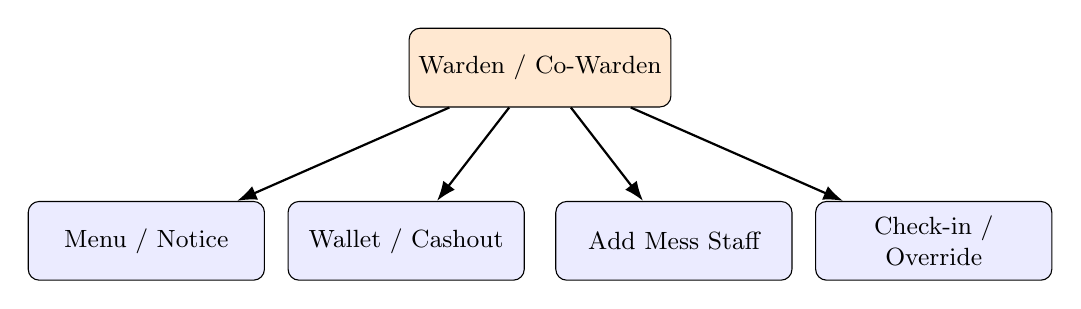
\begin{tikzpicture}
      \node[actor] (warden) at (0, 3)    {Warden / Co-Warden};
      \node[box]   (m1) at (-5, 0.8)  {Menu / Notice};
      \node[box]   (m2) at (-1.7, 0.8) {Wallet / Cashout};
      \node[box]   (m3) at (1.7, 0.8)  {Add Mess Staff};
      \node[box]   (m4) at (5, 0.8)   {Check-in /\\Override};
      \draw[flow] (warden) -- (m1);
      \draw[flow] (warden) -- (m2);
      \draw[flow] (warden) -- (m3);
      \draw[flow] (warden) -- (m4);
    \end{tikzpicture}
    \caption{Hostel-Administrator Activities}
    \label{fig:warden}
\end{figure}

Counter (Mess) Staff have a single activity: serve / check-in students at
the counter.

\begin{figure}[h!]
    \centering
    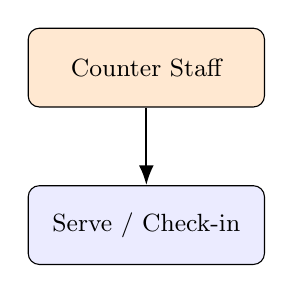
\begin{tikzpicture}
      \node[actor] (staff) at (0, 2) {Counter Staff};
      \node[box]   (serve) at (0, 0) {Serve / Check-in};
      \draw[flow] (staff) -- (serve);
    \end{tikzpicture}
    \caption{Counter Staff Activities}
    \label{fig:staff}
\end{figure}

% ============================================================
\chapter{System Features}
Savoury is a per-meal booking, attendance, and wallet-billing system.
The core of the product is to plan meals, capture who actually eats, and
bill prepaid wallets accurately.

\section{Description and Priority}
Features in priority order (high to low):
\begin{enumerate}
    \item \textbf{Booking \& Opt-out} : the goal feature. Students opt in/out
    of meals before a configurable, IST-based cutoff; a cron job locks
    bookings once the cutoff passes.
    \item \textbf{Attendance \& Billing} : counter staff mark students served;
    each serve writes an attendance row and debits the wallet by the
    per-meal rate in one transaction. Duplicate serves are rejected.
    \item \textbf{Headcount} : live expected-vs-served counts per meal, with
    status (Upcoming / Final / Active / Over) for the kitchen.
    \item \textbf{Wallet} : top-ups by wardens, automatic meal deductions, and
    semester-end cashout requests and approvals.
    \item \textbf{Menu \& Notices} : hostel-scoped menu planning and
    announcements.
    \item \textbf{User \& Role Management} : hostel creation, administrator
    appointment, and per-hostel staff/student management.
\end{enumerate}

\section{Functional Requirements}
Savoury is built on a TypeScript stack across three components.

\textbf{Back-End} : Node.js, Express, TypeScript, Prisma ORM, JWT auth,
Zod validation, node-cron.

\textbf{Front-End (Web)} : React, Vite, React Router, TanStack Query
(admin / warden / staff console).

\textbf{Front-End (Mobile)} : React Native, Expo, Expo Router, TanStack
Query (student app).

\textbf{Database} : PostgreSQL (Supabase).

\medskip
Representative API capabilities (REST):

\begin{longtable}{>{\raggedright\arraybackslash}p{4cm} p{9.5cm}}
\textbf{Area} & \textbf{Functions} \\ \hline
\endhead
Auth & First-admin setup, student registration (college email), login (JWT). \\
Users & Create/update/delete users, change roles, per-hostel scoping and caps. \\
Hostels & Create hostels and fee plans (Super Admin). \\
Menu & View menus (all); create/update menus (committee, hostel admins). \\
Bookings & List bookings, toggle opt-in/out, per-meal headcount. \\
Opt-outs & Batch day-level opt-out / opt-in across date ranges. \\
Attendance & Roster, mark-served / check-in, override (with reason). \\
Wallet & View wallet/transactions, top-up, cashout request/resolve. \\
Notices & List / create / delete hostel-scoped notices. \\
Config & Read / set the semester-end date. \\
\end{longtable}

% ============================================================
\chapter{Other Nonfunctional Requirements}

\section{Performance Requirements}
Headcount and roster queries must return quickly during peak meal times;
the schema is indexed for per-meal headcount and per-student history.
Attendance marking and wallet debit occur inside a single database
transaction to guarantee consistency. A rate limiter protects the API
(a generous global limit for normal app usage and a strict limit on
authentication endpoints).

\section{Security Requirements}
Only authenticated users may access protected endpoints. Passwords are
hashed with bcrypt; sessions use signed JWTs with a 7-day expiry.
Authorization is role-based and hostel-scoped: non-super-admin users act
only within their own hostel, and sensitive actions (role changes,
cashout approvals, overrides) are restricted to the appropriate roles.
Student registration is restricted to the institute email domain.

\section{Software Quality Attributes}
\begin{itemize}
  \item \textbf{Maintainability} : layered architecture
  (routes to middleware to controllers to services to Prisma) with a
  single source of truth for roles.
  \item \textbf{Reliability} : transactional billing and unique constraints
  prevent double-charging and duplicate serves.
  \item \textbf{Testability} : automated tests cover authentication and the
  cutoff logic; the API returns structured errors.
  \item \textbf{Usability} : distinct, time-aware status badges and live
  counts guide staff during service.
\end{itemize}

\section{Business Rules}
Savoury records who eats each meal and bills prepaid wallets accurately,
per hostel. Each hostel has one Warden and one Co-Warden and any number
of Caretakers and Mess Staff. A student is billed only for meals they are
served; opting out before cutoff avoids the charge. Cashout of the
remaining balance is permitted only after the semester-end date.

% ============================================================
\chapter{Other Requirements}
Savoury requires ongoing maintenance as an operational system: periodic
dependency updates, database migrations for schema changes, and
timezone-correct cutoff configuration (times are configured in IST).
Reserved entities (guest meals, feedback, audit log) are present in the
data model for future features and may be enabled as requirements evolve.

\appendix
\chapter{Appendix A: Constraints}
\begin{itemize}
  \item One mess per hostel (MVP); multi-mess support is deferred.
  \item Meal cutoff and serving times are configured as IST wall-clock
  times; meal dates are stored at UTC midnight.
  \item Exactly one Warden and one Co-Warden per hostel; unlimited
  Caretakers and Mess Staff.
  \item Mess Staff do not use the mobile app and are created by
  Wardens/Co-Wardens.
  \item Student accounts require a valid institute email and a hostel.
\end{itemize}

\end{document}
